% \documentclass[11pt, twocolumn]{article}
\documentclass[11pt]{article}   
\usepackage{algorithm2e}
\usepackage[usenames]{color}
\usepackage{lineno}

\usepackage{geometry}                		% See geometry.pdf to learn the
\usepackage{fixltx2e}
\geometry{a4paper}                   		% ... or a4paper or
\usepackage{amsmath}
\usepackage{amssymb}
\usepackage{color}
\usepackage{lineno}
\usepackage{subfigure}
\usepackage[font={bf,small},labelsep=colon]{caption}
\usepackage{authblk}
\usepackage{booktabs}               % For drawing a table
\usepackage[sort]{cite}


\usepackage{graphicx}				% Use pdf, png, jpg, or eps§
\usepackage{hyperref}
\usepackage{fullpage}
\newcommand{\overbar}[1]{\mkern 1.5mu\overline{\mkern-1.5mu#1\mkern-1.5mu}\mkern 1.5mu}
\usepackage{listings}
\lstset{
language=C,
basicstyle=\ttfamily\footnotesize
% basicstyle=\ttfamily\scriptsize
}
\usepackage{multirow}

\newcommand*{\TitleFont}{%
       \usefont{\encodingdefault}{\rmdefault}{b}{n}%
       \fontsize{14}{14}%
       \selectfont}
\newcommand\abs[1]{\left|#1\right|} % Defination of absolute value

\newcommand*\patchAmsMathEnvironmentForLineno[1]{%
  \expandafter\let\csname old#1\expandafter\endcsname\csname #1\endcsname
  \expandafter\let\csname oldend#1\expandafter\endcsname\csname end#1\endcsname
  \renewenvironment{#1}%
     {\linenomath\csname old#1\endcsname}%
     {\csname oldend#1\endcsname\endlinenomath}}% 
\newcommand*\patchBothAmsMathEnvironmentsForLineno[1]{%
  \patchAmsMathEnvironmentForLineno{#1}%
  \patchAmsMathEnvironmentForLineno{#1*}}%
\AtBeginDocument{%
\patchBothAmsMathEnvironmentsForLineno{equation}%
\patchBothAmsMathEnvironmentsForLineno{align}%
\patchBothAmsMathEnvironmentsForLineno{flalign}%
\patchBothAmsMathEnvironmentsForLineno{alignat}%
\patchBothAmsMathEnvironmentsForLineno{gather}%
\patchBothAmsMathEnvironmentsForLineno{multline}%
}

\renewcommand{\baselinestretch}{1.2}

 \title{Derivation of fluid-particle flow equations in lammpsFoam}

\author[1]{Rui Sun}
\author[1]{Heng Xiao\thanks{Email: hengxiao@vt.edu}}

\affil[1]{Department of Aerospace and Ocean Engineering, Virginia Tech, Blacksburg, Virginia, USA}

\renewcommand\Authands{ and }

\date{}
\begin{document}

\maketitle
\tableofcontents

\section{Introduction}
\label{sec:intro}

In CFD--DEM simulations, the fluid volume fraction has to be considered when solving the momentum
equation. This will make the simulation of fluid motion different from solving the original
Navier--Stokes Equation. Anderson and Jackson~\cite{anderson67fm} derived the fluid phase momentum
equations of particle-laden flow, and some people used their equation to perform numerical
simulations and obtained very good results~\cite{xiao11ai}. This document aims at showing how the
CFD--DEM solver lammpsFoam works when solving the fluid phase equations.

\section{Derivation of the equations}

\subsection{Fluid Phase Momentum Equations}
The derivation of the fluid phase momentum equation can be seen in the study of Xiao et
al.~\cite{xiao11ai} and Kafui et al.~\cite{kafui02dp}. Both simulations are based on the derivation
of Anderson and Jackson~\cite{anderson67fm}:
\begin{equation}
  \frac{\partial (\varepsilon_f \rho_f u_i)}{\partial t}
  +\frac{\partial (\varepsilon_f \rho_f u_i u_j)}{\partial x_j} = 
  - \frac{\partial p}{\partial x_i}
  + \frac{\partial}{\partial x_j}\left(\mu \frac{\partial u_i}{\partial x_j}\right)
  + \varepsilon_f \rho_f g_i
  - f_{i,fp}
\label{eqn:NS-DEM-fluid}
\end{equation}
the fluid-particle interaction force by volume $f_{i,fp}$ is:
\begin{equation}
  f_{i,fp} = -\varepsilon_s \frac{\partial p}{\partial x_i} +
  \varepsilon_s\frac{\partial}{\partial x_j}\left(\mu \frac{\partial u_i}{\partial x_j}\right)
  + n \varepsilon_f f_{i,drag}/V_{c}
\label{eqn:NS-DEM-ffp}
\end{equation}
Here, $n$ is the number of particles in the CFD cell, $V_{c}$ is the volume of CFD cell.

When the fluid-particle interaction force in Eq.~(\ref{eqn:NS-DEM-ffp}) is plugged into
Eq.~(\ref{eqn:NS-DEM-fluid}), we have (mentioned in Xiao et al.~\cite{xiao11ai} (2.8)):
\begin{equation}
  \begin{split}
  \frac{\partial (\varepsilon_f \rho_f u_i)}{\partial t}
  &+\frac{\partial (\varepsilon_f \rho_f u_i u_j)}{\partial x_j} = \\
  &- \varepsilon_f \frac{\partial p}{\partial x_i}
   + \varepsilon_f \frac{\partial}{\partial x_j}\left(\mu \frac{\partial u_i}{\partial x_j}\right)
   + \varepsilon_f \rho_f g_i
   - \varepsilon_f \sum\limits_{i=1}^{c_n}f_{i,drag}/V_c 
  \end{split}
\label{eqn:NS-DEM-plugged-xiao}
\end{equation}

In Kafui et al.'s study~\cite{kafui02dp}, the momentum equation is obtained differently:
\begin{equation}
  \begin{split}
  \frac{\partial (\varepsilon_f \rho_f u_i)}{\partial t}
  &+\frac{\partial (\varepsilon_f \rho_f u_i u_j)}{\partial x_j} = \\
  &- \varepsilon_f \frac{1}{\rho}\frac{\partial p}{\partial x_i}
  + {\color{red}\frac{\partial}{\partial x_j}\left(\mu \varepsilon_f \frac{\partial u_i}{\partial
  x_j}\right)}
   + \varepsilon_f \rho_f g_i
   - \varepsilon_f \sum\limits_{i=1}^{c_n}f_{i,drag}/V_c 
  \end{split}
\label{eqn:NS-DEM-plugged-kafui-1}
\end{equation}

Moreover, Kafui et al. combined the drag force with part of the pressure term in his paper:
\begin{equation}
  \frac{\partial (\varepsilon_f \rho_f u_i)}{\partial t}
  +\frac{\partial (\varepsilon_f \rho_f u_i u_j)}{\partial x_j} = 
  - \frac{\partial p}{\partial x_i}
  + \frac{\partial}{\partial x_j}\left(\mu \varepsilon_f \frac{\partial u_i}{\partial x_j}\right)
  + \varepsilon_f \rho_f g_i
  - f_{i,drag,kafui}
\label{eqn:NS-DEM-plugged-kafui-2}
\end{equation}

Since 
\begin{equation}
  f_{i,drag,Kafui} = 
  - (1-\varepsilon_f) \frac{\partial p}{\partial x_i}
  + \varepsilon_f \sum\limits_{i=1}^{c_n}f_{i,drag}/V_c,
\label{eqn:NS-DEM-plugged-kafui}
\end{equation}
Eq.~(\ref{eqn:NS-DEM-plugged-kafui-1}) and Eq.~(\ref{eqn:NS-DEM-plugged-kafui-2}) are theoretically
equivalent equations in different forms. Here, the author of this handbook is still not sure about
the derivation of Kafui et al when dealing with the stress tensor. However, the fluid momentum
equation Kafui et al.  used~\cite{kafui02dp} is the same as the equations used to describe the
motion of multipahse Eulerian flow~\cite{ishii75tf}. 

\subsection{Multiphase Flow in OpenFOAM}
lammpsFoam is based on the Ph.D. thesis of H. Rusche, following the equation for fluid phase
velocity proposed by Ishii~\cite{ishii75tf} and Kafui et al.~\cite{kafui02dp}. The L.H.S. of the
equation, using to describe the fluid motion, is:
\begin{equation}
    \begin{split}
      \frac{\partial (\varepsilon_f \rho_f u_i)}{\partial t}
    &+\frac{\partial (\varepsilon_f \rho_f u_i u_j)}{\partial x_j} - \\
       \left(u_i \frac{\partial (\varepsilon_f \rho_f)}{\partial t}\right.
    &\left.+ u_i \frac{\partial (\varepsilon_f \rho_f u_j)}{\partial x_j} 
     + \varepsilon_f \rho_f \frac{\partial u_i}{\partial t}
     + \varepsilon_f \rho_f u_j \frac{\partial u_i}{\partial x_j}\right)
    \end{split}
\label{eqn:NS-DEM-Rusche-1}
\end{equation}

From the mass conservative equation:
\begin{equation}
    \frac{\partial (\varepsilon_f \rho_f)}{\partial t}
  + \frac{\partial (\varepsilon_f \rho_f u_i)}{\partial x_i} = 0
\label{eqn:NS-DEM-mass}
\end{equation}

We have:
\begin{equation}
    \begin{split}
      \frac{\partial (\varepsilon_f \rho_f u_i)}{\partial t}
    + \frac{\partial (\varepsilon_f u_i u_j)}{\partial x_j} =
      {\color{red}\varepsilon_f \rho_f \frac{\partial u_i}{\partial t}}
    + {\color{red}+\varepsilon_f \rho_f u_j \frac{\partial u_i}{\partial x_j}}
    \end{split}
\label{eqn:NS-DEM-Rusche-eq}
\end{equation}

Then,
\begin{equation}
    \begin{split}
    {\color{red}\varepsilon_f \rho_f \frac{\partial u_i}{\partial t}}
    &{\color{red}+\varepsilon_f \rho_f u_j \frac{\partial u_i}{\partial x_j}} - \\
     \left(- \varepsilon_f \frac{\partial p}{\partial x_i}\right.
    &\left.+ \varepsilon_f \frac{\partial}{\partial x_j}
     \left(\mu \frac{\partial u_i}{\partial x_j}\right)
     + \frac{\partial u_i}{\partial x_j}\frac{\partial}{\partial x_j}\left(\mu \varepsilon_f \right)
     + \varepsilon_f \rho_f g_i
     - \varepsilon_f \sum\limits_{i=1}^{c_n}f_{i,drag}/V_c\right) .
    \end{split}
\label{eqn:NS-DEM-Rusche-2}
\end{equation}

If we divide both sides of Eq.~(\ref{eqn:NS-DEM-Rusche-2}), by $\varepsilon_f \rho_f$, we have:
\begin{equation}
    \begin{split}
    {\color{red}\frac{\partial u_i}{\partial t}}
    &{\color{red}+ u_j \frac{\partial u_i}{\partial x_j}} - \\
     \left(- \frac{1}{\rho_f}\frac{\partial p}{\partial x_i}\right.
    &\left.+ \frac{\partial}{\partial x_j}\left(\nu \frac{\partial u_i}{\partial x_j}\right)
     + \frac{1}{\varepsilon_f}\frac{\partial u_i}{\partial x_j}
       \frac{\partial}{\partial x_j}\left(\nu \varepsilon_f \right)
     + g_i
     - \frac{1}{\rho_f}\sum\limits_{i=1}^{c_n}f_{i,drag}/V_c\right) .
    \end{split}
\label{eqn:NS-DEM-Rusche-3}
\end{equation}
It is equivalent with the equation (3.26) proposed by Rusche.

The code of lammpsFoam (if the turbulence is added) is in a consistent form with
Eq.~(\ref{eqn:NS-DEM-Rusche-3}):
\begin{lstlisting}[basicstyle=\ttfamily\scriptsize]
UbEqn =
(
    (scalar(1) + Cvm*rhob*alpha/rhob)*
    (
        fvm::ddt(Ub)
      + fvm::div(phib, Ub, "div(phib,Ub)")
      - fvm::Sp(fvc::div(phib), Ub)
    )

  - fvm::laplacian(nuEffb, Ub)
  + fvc::div(Rcb)

  + fvm::div(phiRb, Ub, "div(phib,Ub)")
  - fvm::Sp(fvc::div(phiRb), Ub)

  + (fvc::grad(beta)/(fvc::average(beta) + scalar(0.001)) & Rcb)
 ==
//  g  //  Buoyancy term transfered to p-equation
  - fvm::Sp(dragCoef/rhob, Ub)
//  Explicit drag transfered to p-equation
//+ alpha/rhob*dragCoef*Ua 
  + alpha/rhob*(liftCoeff + Cvm*rhob*DDtUa)
);
\end{lstlisting}

The second half of UEqn.H is the expression of various forces of in the simulations. The top half
of UEqn.H can be interpreted as:
\begin{equation}
    \begin{split}
      \frac{\partial u_i}{\partial t}
      + \frac{\partial (u_i u_j)}{\partial x_j}
      - u_i \frac{\partial u_j}{\partial x_j}
      - \frac{\partial}{\partial x_j}\left(\nu_{eff} \frac{\partial u_i}{\partial x_j}\right)
      + \frac{\partial R^c_{ij}}{\partial x_j}\\ 
      + \frac{\partial}{\partial x_j}\left(u_i\frac{-\nu_{eff}}{\varepsilon_f}
        \frac{\partial \varepsilon_f}{\partial x_j}\right)
      - u_i \frac{\partial}{\partial x_j}\left(\frac{-\nu_{eff}}{\varepsilon_f}
        \frac{\partial \varepsilon_f}{\partial x_j}\right)
        + \frac{1}{\varepsilon_f}\frac{\partial \varepsilon_f}{\partial x_j}R^c_{ij}
    \end{split}
\label{eqn:lammpsFoam-1}
\end{equation}

which is equivalent to:
\begin{equation}
    \begin{split}
      \frac{\partial u_i}{\partial t}
      + u_j \frac{\partial u_i}{\partial x_j}
      - \frac{\partial}{\partial x_j}\left(\nu_{eff} \frac{\partial u_i}{\partial x_j}\right)
      + \frac{\partial R^c_{ij}}{\partial x_j}\\ 
      - \frac{1}{\varepsilon_f}\frac{\partial \varepsilon_f}{\partial x_i}
        \nu_{eff}\frac{\partial u_i}{\partial x_j}
      + \frac{1}{\varepsilon_f}\frac{\partial \varepsilon_f}{\partial x_i}R^c_{ij}
    \end{split}
\label{eqn:lammpsFoam-2}
\end{equation}

Eq.~(\ref{eqn:lammpsFoam-2}) is also equivalent to:
\begin{equation}
    \begin{split}
      \frac{\partial u_i}{\partial t}
      + u_j \frac{\partial u_i}{\partial x_j}
      + \frac{\partial}{\partial x_j}\left(-\nu_{eff} \frac{\partial u_i}{\partial x_j} +
      R^c_{ij}\right)
      + \frac{1}{\varepsilon_f}\frac{\partial \varepsilon_f}{\partial x_i}
        \left(-\nu_{eff}\frac{\partial u_i}{\partial x_j}+R^c_{ij}\right)
    \end{split}
\label{eqn:lammpsFoam-3}
\end{equation}

Rusche took $-\nu_{eff}\frac{\partial u_i}{\partial x_j}+R^c_{ij}$ as the stress tensor.
\begin{equation}
      -\nu_{eff}\frac{\partial u_i}{\partial x_j}+R^c_{ij}
      = \tau_{ij} + R_{ij}
\label{eqn:lammpsFoam-tensor}
\end{equation}
Then we proved the U equation in lammpsFoam is consistent with Eq.~(\ref{eqn:NS-DEM-Rusche-3})
except for the gravity term (The gravity term is moved to the pressure equation).

The code of twoPhaseEulerianFoam is:
\begin{lstlisting}[basicstyle=\ttfamily\scriptsize]
U2Eqn =
(
    fvm::ddt(alpha2, U2)
  + fvm::div(alphaPhi2, U2)
  - fvm::Sp(fvc::ddt(alpha2) + fvc::div(alphaPhi2), U2)
  + phase2.turbulence().divDevReff(U2)
 ==
  - fvm::Sp(dragCoeff/rho2, U2)
  + (
        liftForce
      + wallLubricationForce
      + turbulentDispersionForce
    )/rho2
  - virtualMassCoeff/rho2
   *(
        fvm::ddt(U2)
      + fvm::div(phi2, U2)
      - fvm::Sp(fvc::div(phi2), U2)
      - DDtU1
    )
);
mrfZones.addCoriolis(alpha2 + virtualMassCoeff/rho2, U2Eqn);
U2Eqn.relax();
);
\end{lstlisting}

The second half of UEqn.H is the expression of various forces of in the simulations. The top half
of twoPhaseEulerianFoam can be interpreted as:
\begin{equation}
    \begin{split}
      \frac{\partial (\varepsilon_f u_i)}{\partial t}
      + \frac{\partial (\varepsilon_f u_i u_j)}{\partial x_j}
      - u_i \frac{\partial (\varepsilon_f)}{\partial t}
      - u_i \frac{\partial (\varepsilon_f u_j)}{\partial x_j}
      + stress,
    \end{split}
\label{eqn:twoPhase-1}
\end{equation}

which is equivalent to:
\begin{equation}
    \begin{split}
      \varepsilon_f \frac{\partial u_i}{\partial t}
      + \varepsilon_f u_j \frac{\partial u_i}{\partial x_j}
      + stress
    \end{split}
\label{eqn:twoPhase-2}
\end{equation}

Given more studies of the turbulent stress term, this term is mostly taken as
$-\frac{\partial}{\partial x_j}\left(\nu_{eff} \varepsilon_f \frac{\partial u_i}{\partial
x_j}\right)$ instead of $-\varepsilon_f \frac{\partial}{\partial x_j}\left(\nu_{eff} \frac{\partial
u_i}{\partial x_j}\right)$. A further study shows that this difference when dealing with the shear
stress is because of the assumptions of the fluid-solid flow and fluid-fluid flow is different.

\section{Treatment of the stress tensor}

\subsection{Brief Review}

  It seems that the governing equations are different in some CFD--DEM simulations, especially in
  the handling of the stress tensor. There might be no definite answer to this problem, but
  van Wachem et al.'s study~\cite{wachem03mf} may provide some evidence for this open question.

  In van Wachem et al.'s study, Anderson and Jackson~\cite{anderson67fm} derived the continuum
  equations of motion for gas-particle flow. However, Ishii's assumptions of the
  derivation~\cite{ishii75tf} the fluid--fluid governing equations are slightly different, which is
  usually used to study the bubble flow problem. The summary of different forms of equations are
  shown in Fig.~\ref{fig:wachem}
  \begin{figure}[!htbp]
    \centering
      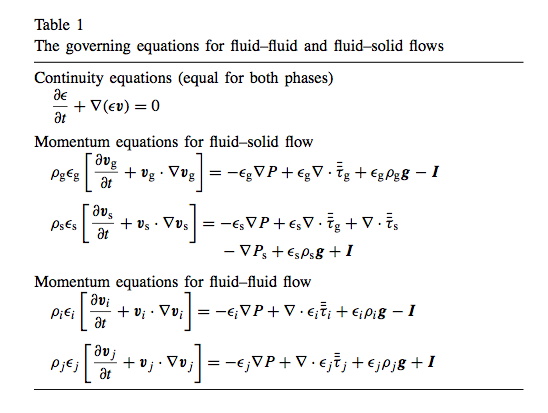
\includegraphics[width=0.8\textwidth]{figs/equations-wachem}
      \caption{ \label{fig:wachem} The equations for fluid--solid flow and fluid--fluid flow
          summarized by van Wachem.}
  \end{figure}

  In van Wachem et al's study, both methods are validated. Despite this, it is only accepted that
  CFD--DEM simulations using $\varepsilon_f \nabla \cdot \tau$ as the stress tensor, and
  fluid--fluid simulations using $\nabla \cdot \varepsilon_f\tau$. However, most CFD--DEM
  simulations do not follow this rule, shown is Table~\ref{tab:sum-fsff}.

  \begin{table}[!htbp]
    \caption{Summary of the fluid--solid and fluid--fluid simulations by different cases
      \label{tab:sum-fsff}}
    \centering
    \begin{tabular}{c|c|c|c|c}
      \hline
      \multirow{2}{*}{author} & \multicolumn{2}{|c}{modeling method} & 
      \multicolumn{2}{|c}{stress tensor}\\\cline{2-5}
      & fluid--solid & fluid--fluid 
      & $\varepsilon_f \nabla \cdot \tau$
      & $ \nabla \cdot \varepsilon_f\tau$ \\
      \hline
      Xiao et al.~\cite{xiao11ai} & \checkmark &  & \checkmark & \\
      A.B. Yu (JFM, 2010) & \checkmark & & \checkmark & \\
      A.B. Yu (CES, 1997) & \checkmark & & & {\color{red}\checkmark} \\
      A.B. Yu (CES, 2007) & \checkmark & & & {\color{red}\checkmark} \\
      Kafui et al.~\cite{kafui02dp} & \checkmark &  &  & {\color{red}\checkmark}\\
      Mueller et al. & \checkmark &  &  & {\color{red}\checkmark}\\
      Rusche~\cite{rusche03cf} & & \checkmark & & \checkmark \\
      bubbleFoam & & \checkmark & & \checkmark \\
      twoPhaseEulerFoam & & \checkmark & & \checkmark \\ 
      \hline
      Tsuji et al. (1993) & \checkmark &  & \multicolumn{2}{c}{ignored}\\
      \hline
    \end{tabular}
  \end{table}

\subsection{Conclusions}
  \begin{enumerate}
    \item CFD--DEM simulations should use $\varepsilon_f \nabla \cdot \tau$ as the stress tensor,
      but in many simulations, people use $\nabla \cdot \varepsilon_f\tau$. In some cases, the
      stress tensor is even ignored.
    \item Both $\varepsilon_f \nabla \cdot \tau$ and $\nabla \cdot \varepsilon_f\tau$ seem acceptable
      in CFD--DEM simulations. In some simulations, the equations derived from Anderson and Jackson
      are directly written as $\nabla \cdot \varepsilon_f\tau$. (See A.B. Yu 1997, Mueller et al.)
    \item Another evidence that both $\varepsilon_f \nabla \cdot \tau$ and $\nabla \cdot
      \varepsilon_f\tau$ are acceptable is: in some of Wachem's simulations, he would even be
      confused with the stress tensor. (See AIChE, 2012) 
    \item In fluid--fluid flow, the stress tensor is mostly taken as $\nabla \cdot
      \varepsilon_f\tau$.
  \end{enumerate}

\section{Large Eddy simulations in OpenFOAM}

Since LES will be implemented in the new lammpsFoam solver, this section serves as an introduction
part. It demonstrates how LES is simulated in OpenFOAM.
% \begin{figure}[!htbp]
%  \centering \includegraphics[width=0.8\textwidth]{figs/figsFinal/diffusion1D_multiple}
%  \caption{ 
%   \label{fig:diffNp}
%   The solution to the diffusion equation with a linear combination of shifted delta functions as
%   initial conditions. The initial condition $\varepsilon(\tau=0)$ is obtained from the procedure of
%   the PCM; $\varepsilon_i(\tau=T)$ are the diffused solutions corresponding to each shifted delta
%   functions; \(\varepsilon(T)\) is the superposition of \(N_p\) Green's functions, which is the
%   result obtained with the proposed coarse graining procedure.}
% \end{figure}

\subsection{Introduction}

  Let's start from Navier--Stokes Equations:
  \begin{equation}
    \frac{\partial u_i}{\partial t}+\frac{\partial u_i u_j}{\partial x_j} = 
    - \frac{1}{\rho}\frac{\partial p}{\partial x_i}
    + \frac{\partial}{\partial x_j}\left( \nu\frac{\partial u_i}{\partial x_j}\right).
  \label{eqn:NS}
  \end{equation}

  If the velocity $u$ and the pressure $p$ are filtered, we have:
  \begin{equation}
    \frac{\partial \overbar{u_i}}{\partial t}+\frac{\partial \overbar{u_i u_j}}{\partial x_j} = 
    - \frac{1}{\rho}\frac{\partial \overbar{p}}{\partial x_i}
    + \frac{\partial}{\partial x_j}\left( \nu\frac{\partial \overbar{u_i}}{\partial x_j}\right).
  \label{eqn:NS-filtered}
  \end{equation}

  If we define the residual stress tensor $\tau_{ij} = \overbar{u_i}\overbar{u_j} - \overbar{u_i
  u_j}$, we have
  \begin{equation}
    \frac{\partial \overbar{u_i}}{\partial t}
    +\frac{\partial \overbar{u_i} \overbar{u_j}}{\partial x_j} = 
    - \frac{1}{\rho}\frac{\partial \overbar{p}}{\partial x_i}
    + \frac{\partial}{\partial x_j}\left( \nu\frac{\partial \overbar{u_i}}{\partial x_j}\right)
    + \frac{\partial \tau_{ij}}{\partial x_j}.
  \label{eqn:NS-decom}
  \end{equation}
  Usually, we employ Boussinesq hypothesis and 
  \begin{equation}
    \tau_{ij}-\frac{1}{3}\tau_{kk}\delta_{ij} = 2 \nu_t \overbar{S_{ij}},
  \label{eqn:NS-tauij}
  \end{equation}
  Where $\overbar{S_{ij}} = 1/2 (\partial \overbar{u_i}/\partial x_j + \partial
  \overbar{u_j}/\partial x_i)$. Then we have:
  \begin{equation}
    \frac{\partial \overbar{u_i}}{\partial t}
    + \frac{\partial \overbar{u_i}\overbar{u_j}}{\partial x_j} = 
    - \frac{1}{\rho}\frac{\partial \overbar{p}}{\partial x_i}
    + \frac{\partial}{\partial x_j}\left([\nu+\nu_t]\frac{\partial \overbar{u_i}}{\partial x_j}\right).
  \label{eqn:NS-LES}
  \end{equation}
  In this case, the pressure is modified to include the trace term $-1/3\tau_{kk}\delta_{ij}$.

\subsection{Filtered Navier--Stokes Equations in OpenFOAM}

In pisoFoam.C, we have:
    \begin{lstlisting}
     fvVectorMatrix UEqn
     (
         fvm::ddt(U)
       + fvm::div(phi, U)
       + turbulence->divDevReff(U)
     );
    \end{lstlisting}
In a representative LES model, say GenEddyVisc.C, we have:
    \begin{lstlisting}
    tmp<fvVectorMatrix> 
    GenEddyVisc::divDevReff(volVectorField& U) const
    {
        return
        (
          - fvm::laplacian(nuEff(), U)
          - fvc::div(nuEff()*dev(T(fvc::grad(U))))
        );
    }
    \end{lstlisting}

Since the term:
    \begin{lstlisting}
        - fvc::div(nuEff()*dev(T(fvc::grad(U))))
    \end{lstlisting}
will be zero if the fluid mass is conservative (see derivation), we have:
    \begin{lstlisting}
     fvVectorMatrix UEqn
     (
         fvm::ddt(U)
       + fvm::div(phi, U)
       - fvm::laplacian(nuEff(), U)
     );
    \end{lstlisting}
which is consistent with Eq.~(\ref{eqn:NS-LES}).


\subsection{Subgrid scale modeling}

According to the study performed by Fureby et al.~\cite{fureby97ac}, the SGS stress
  tensor is represented as:
  \begin{equation}
  \begin{split}
    \tau_{ij} & = \frac{2}{3}kI_{ij}-2\nu_tS_{ij,D},\\
    k & = \frac{1}{2}\mathrm{tr}(\tau_{ij}), 
    S_{ij,D}=S_{ij}-\frac{1}{3}\mathrm{tr}(S_{ij})I_{ij}
  \label{eqn:tau_sgs}
  \end{split}
  \end{equation}
  According to Smagorinsky model,
  \begin{equation}
    k=c_I\Delta^2|S_{ij}|^2, \nu_t=c_D\Delta^2|S_{ij}|,
  \label{eqn:sma-tau}
  \end{equation}
  Then the SGS stress tensor can be modeled.

  Here is how the SGS model in implemented in OpenFOAM
    \begin{lstlisting}
        B = 2/3*k*I - 2*nuSgs*dev(D)
        Beff = 2/3*k*I - 2*nuEff*dev(D)

        D = symm(grad(U));
        k = (2*ck/ce)*delta^2*||D||^2
        nuSgs = ck*sqrt(k)*delta
        nuEff = nuSgs + nu
    \end{lstlisting}
  The defination of $k$ and $\nu_t$ are the same as the reference since:
    \begin{equation}
        \begin{split}
        \nu_t &= c_k\sqrt{2c_k/c_e}\Delta^2|S_{ij}|,\\
        c_D &= c_k\sqrt{2c_k/c_e} \approx 0.042.
        \end{split}
    \label{eqn:sma-eqav}
    \end{equation}
  It is also consistent with Pope's defination~\cite{pope00tf}. (The $c_D$ recommended by Pope is
  0.028, but it is because the definations of $|S_{ij}|$ are not consistent in both studies. The
  equations for $\nu_t$ are consistent.) The SGS model in OpenFOAM is consistent with the turbulent
  theories.

\subsection{LES--DEM Equations}

  From Fang et al.'s work~\cite{fang13li} (I copied the original equations):
  \begin{equation}
    \frac{\partial \left(\overbar{\varepsilon}\overbar{u_i}\right)}{\partial t}
    +\frac{\partial \left(\overbar{\varepsilon}\overbar{u_i} 
     \overbar{u_j}\right)}{\partial x_j} = 
    - \frac{1}{\rho}\frac{\partial \overbar{p}}{\partial x_i}
    + \frac{\partial}{\partial x_i}\left(\nu\frac{\left(\partial 
      \overbar{\varepsilon}\overbar{u_i}\right)}{\partial x_j}\right)
      + \frac{1}{\rho}\frac{\partial \left(\overbar{\varepsilon}\tau_{ij}\right)}{\partial x_j}.
  \label{eqn:NS-DEM-filtered}
  \end{equation}
  the sub-grid stress tensor is taken as:
  \begin{equation}
    \tau_{ij}-\frac{1}{3}\tau_{kk}\delta_{ij} = 2 \mu_t \overbar{S_{ij}},
  \label{eqn:NS-DEM-tauij}
  \end{equation}
  Where $\overbar{S_{ij}} = 1/2 (\partial \overbar{u_i}/\partial x_j + \partial
  \overbar{u_j}/\partial x_i)$. The turbulent viscosity is defined as:
  \begin{equation}
    \nu_t = (C_s \Delta)^2\sqrt{2\overbar{S_{ij}}\overbar{S_{ij}}}.
  \label{eqn:NS-LES-2}
  \end{equation}

  In my perspective, there might be a few mistakes in the equations:
  The correct form of Navier--Stokes equations is:
  \begin{equation}
    \frac{\partial \overbar{\varepsilon}\overbar{u_i}}{\partial t}
    +\frac{\partial \overbar{\varepsilon}\overbar{u_i} \overbar{u_j}}{\partial x_j} = 
    - \frac{1}{\rho}\frac{\partial \overbar{p}}{\partial x_i}
    + \frac{\partial}{\partial {\color{red}x_j}}\left(\nu\frac{\partial 
      \overbar{\varepsilon}\overbar{u_i}}{\partial x_j}\right)
      + \frac{1}{\rho}\frac{\partial \overbar{\varepsilon}\tau_{ij}}{\partial x_j}.
  \label{eqn:NS-DEM-filtered-corrected}
  \end{equation}
  Also, the implementation of this equation is also straightforward.


\section{Useful Advices}
  In the joint group meeting on 09/05/14, Dr. Liu suggested we check the forces added to the
  particles. I looked through the code and noticed that:
\begin{lstlisting}[basicstyle=\ttfamily\scriptsize]
    // local pressure gradient is used though (no weighting).
    pDrag_[particleI] =
        Jd_[particleI]*(1.0 - pAlpha_[particleI])
       *p.Vol()*Uri_[particleI]         // Drag
      - gradp[p.cell()]*p.Vol();        // Buoyancy

\end{lstlisting}
  the drag and buoyancy is added to the particles, but the added mass is not considered. For
  particle--gas flow, the added mass is negligible, but for sediment transport simulations, this is
  not.

  Another useful advice from Dr. Calantoni is that the distribution of bottom particles should not
  be regular. Adding a random height of the particles may help.

\section{Plan for new implementations}
After we talked with Dr. Liu and Dr. Calantoni, we found out that we can still improve the
simulation in several ways.
  \begin{enumerate}
    \item Add the virtual mass force in the particle motion, though it is not considered in
      Schmeeckle's simulations~\cite{schmeeckle14ns}.
    \item Change the initial distribution of the ``frozen'' particles, add a random offset to them.
    \item Verification of the code and validation of the cases.
  \end{enumerate}

  If it is still not working, the turbulence stress should be added.
  \begin{enumerate}
    \item Keep the source code of lammpsFoam. Update it to 2.3.x version.
    \item Change the UEqn part, make it looks like the new version. (The meaning of each term will
      be more explicit after this.) 
    \item Make use of the two-phase turbulence models in 2.3.x version, change the stress tensor in
      lammpsFoam. (The stress tensor in two-phase turbulence models is $\nabla \cdot
      \varepsilon_f\tau$ in OpenFOAM. Improve the two-phase stress tensor to the correct one.)
    \item Verification and Validation.
  \end{enumerate}

\bibliographystyle{unsrt}
\bibliography{twoPhaseModeling}


\end{document}

